\documentclass{article}

\usepackage[brazil]{babel}
\usepackage[utf8]{inputenc}
\usepackage{amsmath}
\usepackage{amsfonts}

\usepackage{listings}
\usepackage{mcode}
\usepackage[section]{placeins}

\usepackage{graphicx}

\usepackage{color} %red, green, blue, yellow, cyan, magenta, black, white
\definecolor{mygreen}{RGB}{28,172,0} % color values Red, Green, Blue
\definecolor{mylilas}{RGB}{170,55,241}

\begin{document}

\begin{flushleft}
FUNDAÇÃO GETÚLIO VARGAS \\

Escola de Pós-Graduação em Economia

Teoria Macroeconômica III

Professor: Ricardo de Oliveira Cavalcanti

Monitora: Kátia Aiko Nishiyama Alves

Alunos: Gustavo Bulhões e Samuel Barbosa
\end{flushleft}

\section*{Exercício 03}

\subsection*{Item (i)}

O problema do planejador é dado por 

\begin{equation}
\begin{aligned}
& \max & & \mathbb{E}_0 \sum_{t=0}^{\infty} \beta^t u(c_t) \\
& \text{s.a.} & &  c_t + k_{t+1} \leq z_t k_t^\alpha + (1-\delta) k_t \\
& & &  k_{t+1} \geq 0, c_t \geq 0 \,\, \forall t \geq 0  \\
& & &  k_0 \text{ dado} \\
\end{aligned}
\end{equation}

\subsection*{Item (ii)}

As variáveis de estado desta economia são $k$ e $z$. Reescrevendo o problema na forma recursiva, temos

\begin{equation}
\begin{aligned}
V(k, z) = & \max_{c, k'} & & u(c) + \beta \sum_j \pi_{ij} V(k', z'_j) \\
& \text{s.a.} & &  c + k' = z k^\alpha + (1-\delta) k \\
& & &  k' \geq 0, c \geq 0 \,\, \\
\end{aligned}
\end{equation}

\subsection*{Item (iii)}

O operador de Bellman associado à equação funcional obtida no item anterior é

\begin{equation}
\begin{aligned}
T(V)(k, z) = & \max_{c, k'} & & u(c) + \beta \sum_j \pi_{ij} V(k', z'_j) \\
& \text{s.a.} & &  c + k' = z k^\alpha + (1-\delta) k \\
& & &  k' \geq 0, c \geq 0 \,\, \\
\end{aligned}
\end{equation}

\subsection*{Item (iv)}

Utilizando os parâmetros e funções dadas, alteramos o código do exercício anterior para
incorporar a incerteza referente aos choques na variável $z$.

\begin{lstlisting}
% Parametros
alpha = 0.70;
beta = 0.98;
gamma = 2.00;
delta = 0.10;

zh = 1.2;
zl = 0.8;

kssh = (1/(zh*alpha)*(1/beta-1+delta))^(1/(alpha-1));
kssl = (1/(zl*alpha)*(1/beta-1+delta))^(1/(alpha-1));

% Funcoes
f = @(k, z) z * k .^ alpha;
c = @(k, k_linha, z) max(f(k, z) + (1 - delta) * k - k_linha, 0);
u = @(c) (c .^ (1 - gamma)) ./ (1 - gamma);

% Grid
n = 1000;
k = linspace(0.7 * kssl, 1.3 * kssh, n);
k_linha = k';
K = repmat(k, n, 1);
K_linha = repmat(k_linha, 1, n);

% Chutes iniciais:
Vzh = zeros(1, n);
Vzl = zeros(1, n);
Gzh = zeros(1, n);
Gzl = zeros(1, n);
z = zh;

% Consumo e utilidade
Ch = c(K, K_linha, zh);
Cl = c(K, K_linha, zl);
Uh = u(Ch);
Ul = u(Cl);

% Variaveis iteracao
err = 1;
tol = 10^-5;
it = 1;
itmax = 1000;

%% Algoritmo de iteracao
while err > tol && it < itmax
    if z == zh
        [TVzh, Izh] = max(Uh + beta * (0.7 * repmat(Vzh',1, n) + 0.3 * repmat(Vzl',1, n)));
        err = max(abs((TVzh - Vzh)));
        Vzh = TVzh;
        x = rand(1);
        if x <= 0.7, z = zh; else z = zl; end
        it = it + 1;
    else
        [TVzl, Izl] = max(Ul + beta * (0.8 * repmat(Vzh',1, n) + 0.2 * repmat(Vzl',1, n)));
        err = max(abs((TVzl - Vzl)));
        Vzl = TVzl;
        it = it + 1;
        x = rand(1);
        if x <= 0.8, z = zh; else z = zl; end
        it = it + 1;
    end
end

Gzh = k(Izh);
Gzl = k(Izl);
\end{lstlisting}

\subsection*{Item (v)}

Executando o código acima obtemos as seguintes funções valor e polítca:

\begin{figure}[!h]
  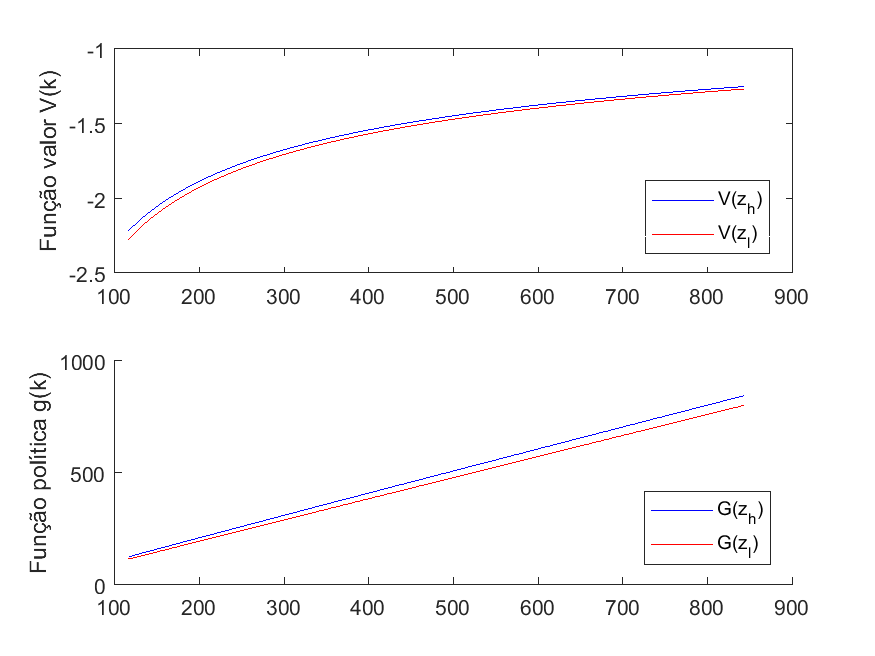
\includegraphics{ex3_1.png}
\end{figure}

\end{document}